\documentclass[11pt]{article}
\usepackage{longtable}
\usepackage{color}
\usepackage{tabu}
\usepackage{setspace}
\usepackage{pdflscape}
\usepackage{graphicx}
\usepackage {float}
%\usepackage{subfigure}
\usepackage{caption}
\usepackage{subcaption}
\usepackage{natbib}
\usepackage{fullpage}
\bibliographystyle{plain}
%\bibliographystyle{cbe}
\usepackage{algorithmic}
\usepackage[vlined,ruled]{algorithm2e}
\usepackage{amsmath}
\usepackage{amsfonts}
\usepackage{amssymb}
\usepackage[T1]{fontenc}
\usepackage{url}
 
\usepackage[dvipsnames]{xcolor}
\usepackage{color, soul}
\usepackage[colorlinks=true, linkcolor=blue, citecolor=DarkOrchid, urlcolor=TealBlue ]{hyperref}
%\usepackage[nottoc,numbib]{tocbibind}
\usepackage{tocloft}


\setlength\itemindent{0.25cm}

\newcommand{\phyg}{\texttt{PhyG} }
\newcommand{\BigO}[1]{\ensuremath{\mathcal{O}\left(\,#1\,\right)}\xspace}

\title{PhyG 0.1 Tutorials}

\author{Louise M. Crowley}
\makeindex
\begin{document}
\maketitle


%Maybe add:\\
%\begin{enumerate}
%	\item{reports of diagnosis}
%	\item{Supports--Goodman-Bremer, bootstrap, jackknife--maybe on chel or 
%	something preassigned and small}
%	\item{Consensus etc outputs}
%\end{enumerate}

\section{\phyg Tutorials}

These tutorials are intended to provide guidance for using the phylogenetic 
program \texttt{PhyG}. Each tutorial contains a \phyg script that includes 
detailed commentaries explaining the rationale behind each step of the analysis. 
The command arguments will differ substantially depending on type, complexity, 
and size of the data set. The values of arguments within this tutorial have been 
chosen such that the analysis can complete within the timeframe of this session.
Therefore, the values used here should not be taken to be optimal parameters. 

The tutorials use sample datasets that can also be downloaded from the \texttt{PhyG} 
\href{https://github.com/amnh/PhyGraph}{GitHub} website. The minimally required 
items to run the tutorial analyses are the \phyg application and sample data files. 
Running these analyses requires some familiarity with the \phyg command structure 
that can be found below (see Section \ref{subsec:Scripts}). A complete guide to the
commands and associated arguments of \phyg can be found 
\href{https://github.com/amnh/PhyGraph}{here}.

%-------------------------------------------------------------------------------------------------------
\subsection{Obtaining and Installing \phyg}
\label{subsec:Installation}

In this tutorial, you will learn how to obtain and install the \phyg binaries.  
Precompiled \phyg binaries, test data, and documentation in pdf format are available 
from the \phyg \href{https://github.com/amnh/PhyGraph}{GitHub} website. 

\begin{enumerate}
\item Open a web browser and navigate to the \phyg \href{https://github.com/amnh/PhyGraph}
{GitHub} website. In the \textit{bin} directory, binaries are available for Mac OSX 
computers with either Intel or M1 processors, and Linux (Intel) machines (see information 
relating to Windows machine below).

\item Click on the appropriate link for the binary. On most systems this will 
download to either your Desktop or Downloads folder. 

\item The user is advised to change the permissions of the binary to ensure
that it is executable. In a terminal window, navigate to the directory where the \phyg
binary is located. Type the following:

	\begin{quote}
	chmod +x phyg
	\end{quote}

\item With Mac OSX machines, right click on the binary, and select `open with 
\textit{Terminal}', and click `Open'. The OSX has now marked the binary as `safe' 
to open. In Linux machines, it is not necessary to mark executables as `safe'.

\item The binary should either be moved into your \$PATH or referred to its 
absolute PATH when executing a script. Your \$PATH is a colon-separated list 
of directories, the contents of which you can execute without specifying the 
absolute path. To find out what's in your \$PATH, open a \textit{Terminal} window 
(located in your Applications folder) and type: 

	\begin{quote}
	echo \$PATH
	\end{quote}

If the directories \texttt{/usr/local} or \texttt{/usr/local/bin} do not exist yet, type the 
following (\texttt{sudo} will require Admin password): 

	\begin{quote}
	sudo mkdir -p /usr/local/bin
	\end{quote}

\item For users without administrative privileges for their computer, save
this binary at your preferred location (for instance in `Applications') and refer to its 
absolute PATH when executing a script: 

	\begin{quote}
  	/Applications/phyg ~/Desktop/phygfiles/run1.pg
	\end{quote}
	
See also below in Subsection \ref{subsec:executing}.
	
\item Move the \phyg binary from its current location to this location. For example 
typing the following will move the binary from its Desktop location into the user's 
\$PATH:

	\begin{quote}
	sudo mv ~/Desktop/phyg /usr/local/bin
	\end{quote}	
	
\item For those users with Windows machines, a Windows Subsystem for Linux 
(WSL) can be installed. This system will allow you to run the Linux binary directly 
on your machine, without having to install a virtual machine or dual-boot setup. 
The WSL, along with directions for installation, can be found 
\href{https://learn.microsoft.com/en-us/windows/wsl/}{here}.
\end{enumerate}

%-------------------------------------------------------------------------------------------------------
\subsection{Making a \phyg script}
\label{subsec:Scripts}

\phyg analyses are conducted using a script and cannot be performed interactively. 
A script is a simple text file containing a list of commands to be performed. \phyg 
scripts can be created and saved using any conventional text editor (such as 
\textit{TextEdit}, \textit{TextWrangler}, \textit{BBEdit}, \textit{Emacs}, or \textit{NotePad}). 
Do not use a word processing application like \textit{Microsoft Word} or \textit{Apple 
Pages}, as these programs can introduce hidden characters in the file, which will be 
interpreted by \phyg and can cause unpredictable parsing of the data. In this tutorial, 
you will learn about the format of \phyg scripts and how to generate one for execution 
by the program.

\begin{enumerate}

\item Open your text editor of choice.

\item Type the following:
	
	\begin{quote}
	-\/-Chel first analysis\\
	set(seed:73412305)\\
	set(outgroup:"Limulus")\\
	read(nucleotide:"chel\_16S.fas")\\
	read(nucleotide:"chel\_cox1.fas")\\
	report("chel\_cr1.csv", crossrefs, overwrite)\\
	report("chel\_data1.csv", data, overwrite)\\
	\end{quote}

Note: the commands \texttt{read}, \texttt{rename}, \texttt{reblock}, and \texttt{set} 
are executed at the beginning of program execution, irrespective of where they 
appear in the command script. All other commands are executed in the order they 
are specified.

\item In this example, the script begins with a comment that describes the 
contents of the file. Comments are prepended with `-{}-' and can span multiple 
lines, provided each line begins with `-{}-'. \phyg will ignore any commented 
lines. Comments can provide useful information to the reader to understand 
the purpose of the script. They can also be useful for testing purposes.

\item Each command consists of a name, followed by a list of arguments or options 
separated by commas and enclosed in parentheses. Commands and arguments are 
case insensitive, with the exception of filename specifications, which are always in 
double quotes (\textbf{"fileName"}). There are defaults for all options except 
input graphs. The command, followed by open and closed parentheses `\texttt{()}',
denotes default options, e.g. \texttt{build()} is the equivalent of \texttt{build(character, 
replicates:10)}.

\item In this script, the seed for the random number generator is \texttt{set} to 
the integer value 73412305. By setting this value, you are guaranteed to reproduce 
a given search strategy each time the script is run. This value can be any number of 
digits in length. Note: this seed value should not be mistaken for the initial random
seed value, as chosen by the application (see Figure \ref{output1}).

\item Next \texttt{set} the outgroup for the analysis to \textit{Limulus}. If the outgroup
is not set, \phyg will sort the taxa alphabetically and choose the first taxon as the
outgroup. Only a single taxon can be set as the outgroup of the analysis. Note: taxon 
names cannot have spaces, otherwise the names can be incorrectly interpreted by
the program.

\item The command \texttt{read} imports file-based information, including data files, 
tree and graph files. \texttt{read} commands must contain an input file. Supported 
data formats include FASTA, FASTC and TNT files, and graph formats include Dot, 
Enewick, and Newick. Filenames must include the suffix (e.g. 
.fas, .fasta, .fastc, .ss, .tre). Failure to include these suffices will result in the error 
"File(s) not found in `read' command". The filename must match \textit{exactly}, 
including capitalization.\\
\\
\texttt{read} also accepts wild cards. The user can use an asterisk (*) to represent 
zero or more characters. For example, to read all the filenames with the extension .fas, 
the user can simply type:
        
        \begin{quote}
	read(nucleotide:"*.fas")\\
	\end{quote}
	
Moreover, to capture all the filetypes ending with fas, the user can type: 
	
	\begin{quote}
	read(nucleotide:"*.fas*")\\
	\end{quote}

This will read files ending in .fas, .fasta, and .fastc. \phyg will attempt to recognize 
the type of input and parse appropriately. Otherwise, the type of file can be 
indicated. In this example, we indicate that the files "chel\_16S.fas" and 
"chel\_cox1.fas" contain IUPAC \texttt{nucleotide} sequence data in fasta format.

\item Having read in our data, it is advisable to verify that the files were properly 
parsed by checking the characters and terminals in the cross-references and data 
files. We will examine these files below (Section \ref{subsec:Inspecting}).

\item Save this file with the name \textbf{run1.pg} in a directory \textbf{phygfiles} 
located on your Desktop. Note: the tutorial data files should be moved to this 
location also.

\end{enumerate}

%-------------------------------------------------------------------------------------------------------
\subsection{Executing scripts}
\label{subsec:executing}

In this tutorial you will learn how to execute a script using \texttt{PhyG}. 

\begin{enumerate}

\item Before we read the data, we will make sure that \phyg is working in the directory 
containing the data files. The working directory tells the application where to look 
for the files. In this way, whenever we tell \phyg to read a file, we don't need to 
specify where it is located in the file system, we can simply use its name. To 
begin, open a \textit{Terminal} window.
        
\item Change the directory to where the script \textbf{run1.pg} is located by using the 
\texttt{cd} command, as in:
		
	\begin{quote}
	cd ~/Desktop/phygfiles
	\end{quote}
   
\item By typing \texttt{ls} you will see that this directory contains the script 
\textbf{run1.pg}.

\item The program is invoked from the command-line, as in:
		
	\begin{quote}
	phyg commandFile
	\end{quote}
	
To run the script \textbf{run1.pg} type the following:
		
	\begin{quote}
  	phyg run1.pg
	\end{quote}
	
This is equivalent to typing the following from any location on your computer:
	
	\begin{quote}
  	phyg ~/Desktop/phygfiles/run1.pg
	\end{quote}

Note: should you get the error ``phyg: command not found'' this indicated that 
\texttt{Phyg} is not in your path. 
	
\item To interrupt the analysis, press control-c. Interrupting the analysis cancels 
the execution of the last command requested by the user. 

\end{enumerate}

%-------------------------------------------------------------------------------------------------------
\subsection{Inspecting the data}
\label{subsec:Inspecting}

In this tutorial you will learn how to inspect data in both the terminal window and 
in reported output files. Running the script will automatically generate an extensive, 
detailed output in the terminal window. It may also be desirable to inspect the 
imported data in greater detail to ensure that the format and contents of the files 
have been interpreted correctly. This practice helps avoid common errors, such 
as inconsistently spelled terminal names, which may result in bogus results, 
produce error messages, and aborted jobs.

\begin{enumerate}

\item Having run the script, examine the output in the terminal window 
(Figure \ref{output1}). \phyg will continue to output information to the screen 
until the completion of the analysis. It is possible to scroll through this output, 
even as the analysis continues to run. The output includes the landing page, 
the name of the script, the random seed, whether the files were 
correctly specified, the name of the input file(s), whether the terminals were 
renamed, whether trees were selected, and a brief description of the content 
for each loaded file. The current state of the analysis can be viewed here. Any 
warnings and errors will also appear here. Upon completion of the analysis, the 
results, including costs, the number of returned graphs, and information relating 
wall-clock time, CPU time, and CPU usage are also provided.

\begin{figure}
\centering
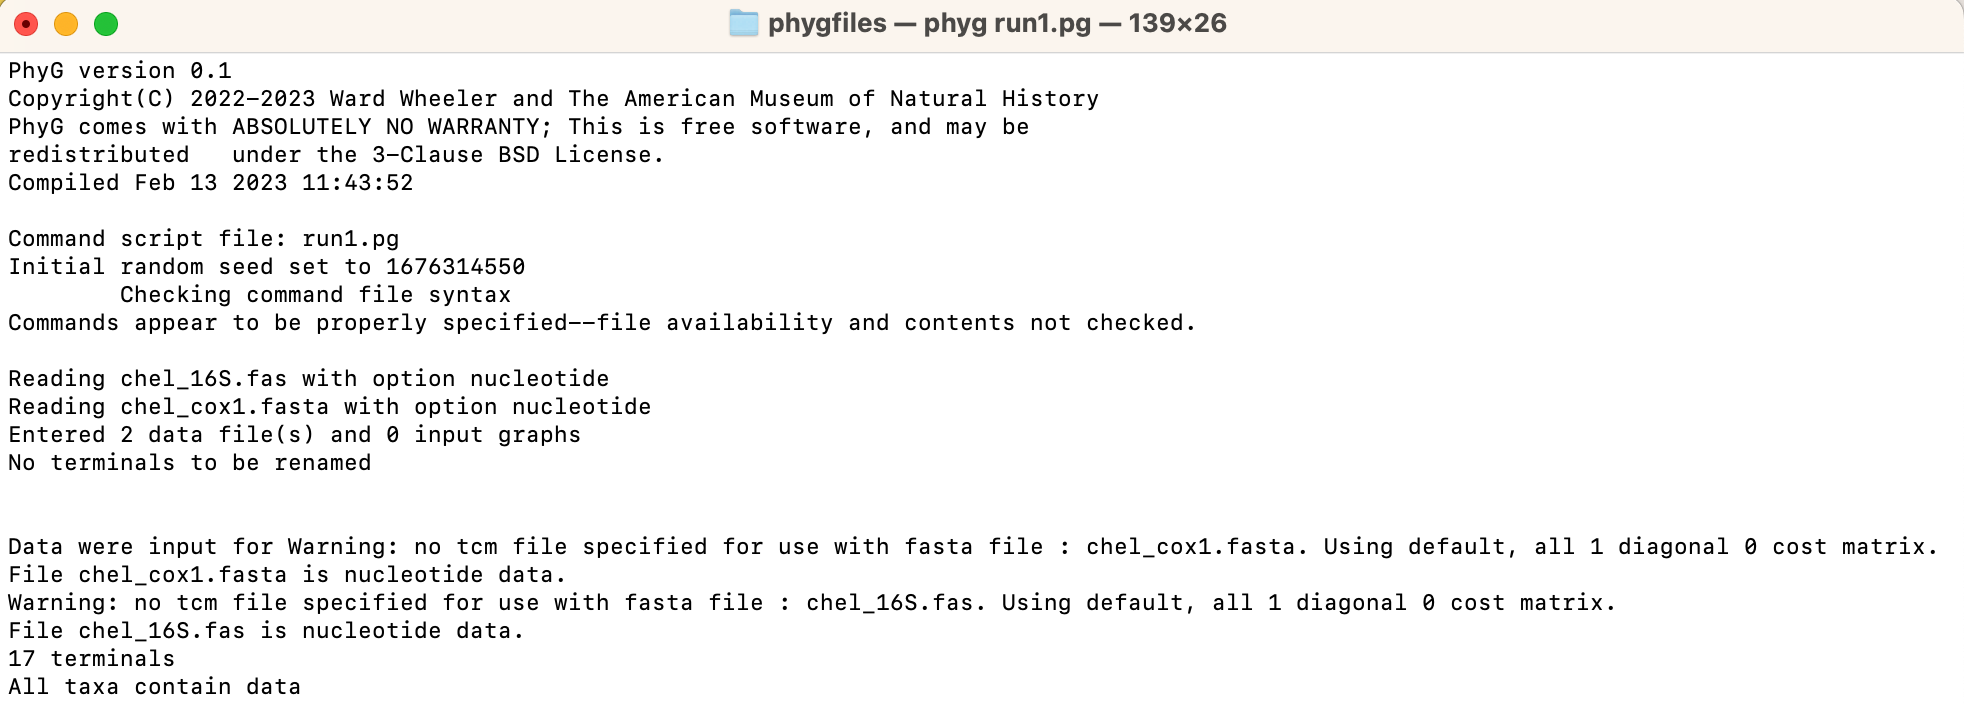
\includegraphics[width=\textwidth]{output1.png}
\caption{The \phyg output display in the \textit{Terminal} window at the beginning 
of an analysis.}
\label{output1}
\end{figure}

\item A good practice is to confirm that \phyg parsed the input files correctly. 
By examining the output in the terminal, you can see that both files were
interpreted and read in as nucleotide sequence data files by the program 
(Figure \ref{output1}).

\item Let's reexamine our script:

	\begin{quote}
	-\/-Chel first analysis\\
	set(seed:73412305)\\
	set(outgroup:"Limulus")\\
	read(nucleotide:"chel\_16S.fas")\\
	read(nucleotide:"chel\_cox1.fas")\\
	report("chel\_cr1.csv", crossrefs, overwrite)\\
	report("chel\_data1.csv", data, overwrite)\\
	\end{quote}
	
Having imported our data files, we next \texttt{report} a crossrefs and data file.
The command \texttt{report} outputs the results of the current analysis or loaded 
data by directing it to a file. To redirect the output to a file, the file name (in quotes), 
followed by a comma, must be included in the argument list of report. All arguments 
for \texttt{report} are optional. This command allows the user to output information 
concerning the characters and terminals, diagnosis, export static homology data, 
implied alignments, trees, graphs, dot files, as well as other miscellaneous arguments. 
By default, new information printed to a file is appended to the file. The option 
\texttt{overwrite} overrides the default and rewrites the file rather than appending 
to the existing information. Many of the report options can be output in csv format, 
which can subsequently be imported into spreadsheet applications like \textit{Excel} 
or \textit{Numbers} for easy viewing. 

\item Examine the reported file \textbf{"chel\_cr1.csv"}. The \texttt{crossrefs} 
argument of the \texttt{report} command is a useful tool for the visual representation 
of the inputted data. This argument displays whether data are present or absent 
for each terminal in each of the imported data files. This provides a comprehensive 
visual overview of the completeness of the data. It will highlight missing data, as 
well as inconsistencies in the spelling of taxon names in different data files (see 
Figure \ref{crossrefs}). The argument will report a file with the terminals represented 
in rows, and the data files in columns. A plus sign ``+'' indicates that data for a given 
terminal is present in the corresponding file; a minus sign ``-'' indicates that it is not.

\item Open the csv file using  your spreadsheet program of choice (Figure \ref{crossrefs}). 
The user is encouraged to report a crossrefs file having imported the data 
into \texttt{PhyG}, especially when working with new datasets. 

\begin{figure}
\centering
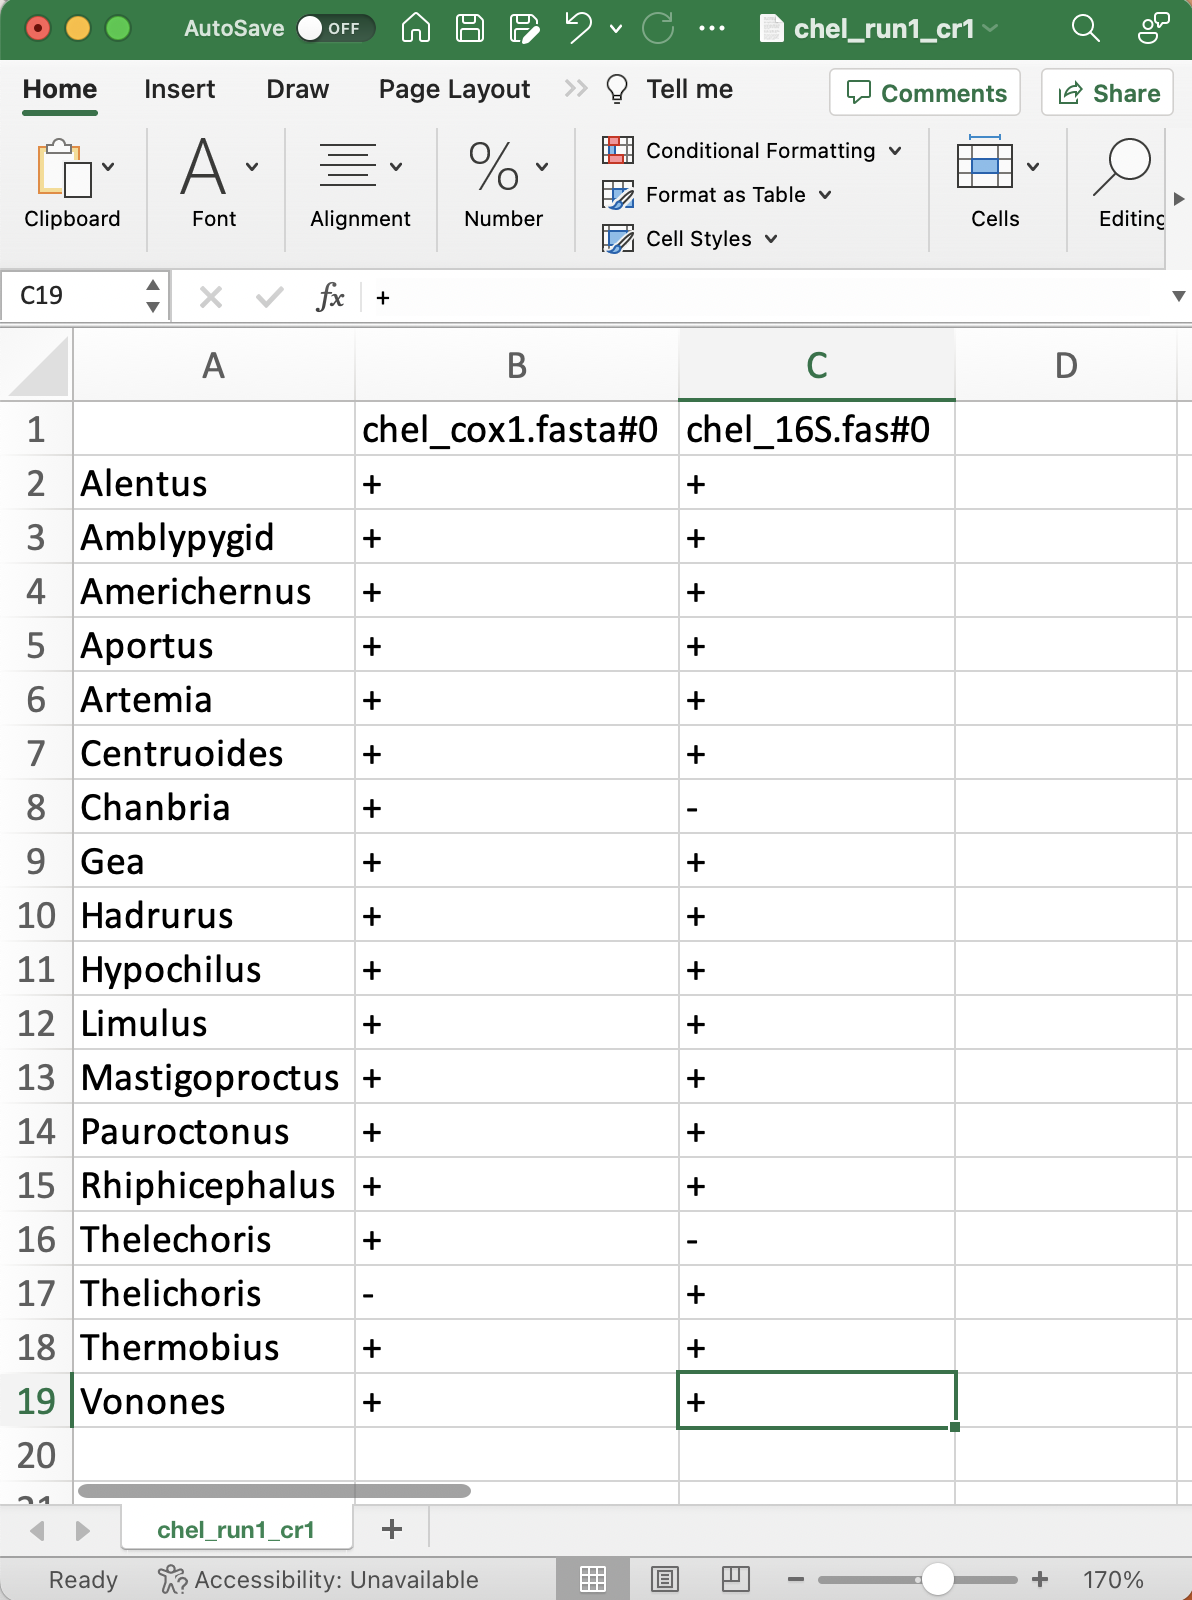
\includegraphics[width=0.45\textwidth]{crossrefs1.png}\hfill
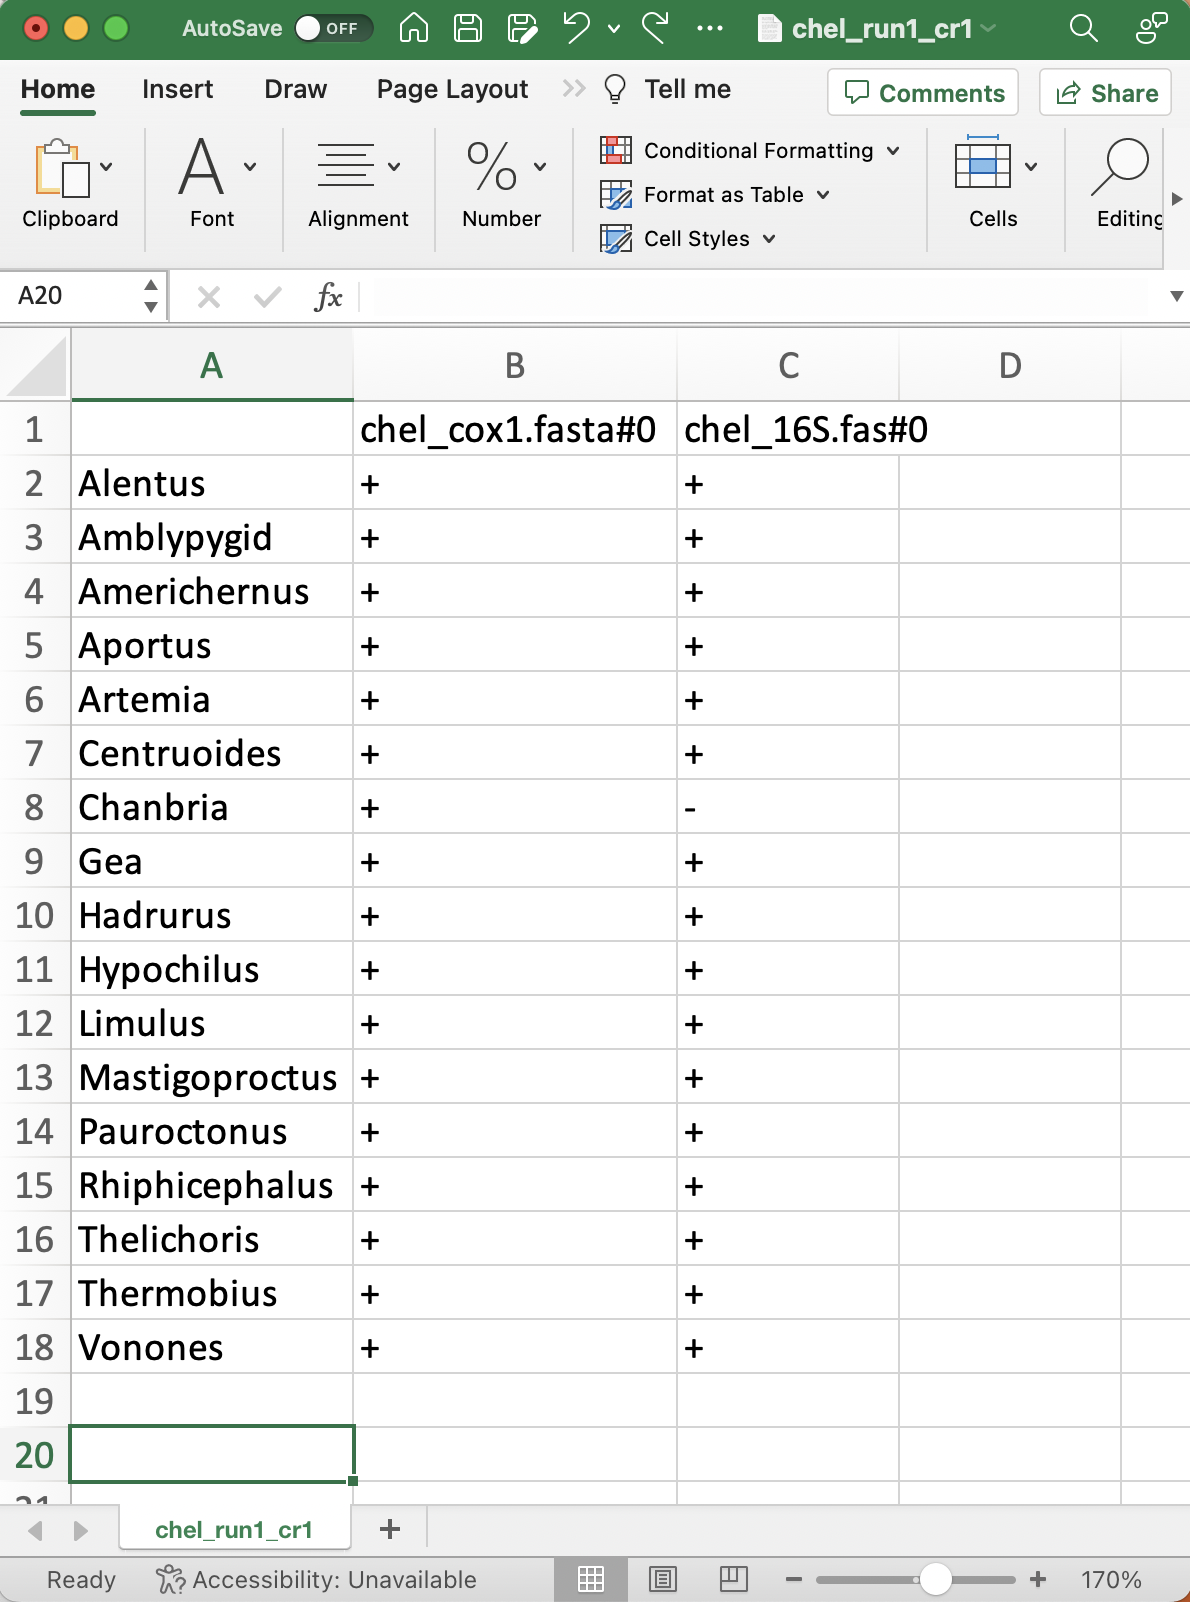
\includegraphics[width=0.45\textwidth]{crossrefs2.png}
\caption{Inspecting imported data. The figure shows two crossrefs files, which have 
been imported into \textit{Excel}. The image on the left illustrates an inconsistency in the 
naming of the taxon \textit{Thelichoris}. This was corrected in the image on the right.}
\label{crossrefs}
\end{figure}
	
\item Examine the reported file \textbf{"chel\_data1.csv"}. This file is a summary 
of different aspects of the input data and terminals. This file summarizes 
information relating to the input data (number of terminals, number of input files, 
number of character blocks and the total number of characters). It also provides
information relating to the terminal taxa included in the analysis, including the 
names of the taxa, a list of the excluded taxa (if any), and whether any terminals 
were renamed. In this file you will also see information relating to 
``Index'', ``Block'', ``Name'', ``Type'', ``Activity'', ``Weight'', ``Prealigned'', ``Alphabet'', 
``TCM''. ``Index'' reports the character number in the overall dataset; ``Name'' the 
name of the character (by default based on its source data file); ``Type'' is the type 
of character (e.g. Non-Additive, Matrix, Nucleotide Sequence), ``Activity'' whether
the character is active (included in the analysis) or not (excluded), ``Weight'' is the 
weight of the character, ``Prealigned''  denotes whether a sequence character 
(e.g. amino acids) is to be treated as prealigned or not, ``Alphabet'' the elements of 
a sequence character, ``TCM'' is the transition cost matrix specifying costs among 
sequence elements and ``gap'' or insertion-deletion.
\end{enumerate}

%-------------------------------------------------------------------------------------------------------
\subsection{Building a tree with nucleotide sequence characters}
\label{subsec:Building}

Having imported and inspected our data, we are now ready to build the initial trees 
or graphs. In this tutorial you will build a distance tree using nucleotide sequence 
characters. The \texttt{build} command builds initial graphs. The arguments of build 
specify the number of graphs to be generated, and whether the build is based on 
distance or character methods. Distance methods are considerably faster, but 
approximate in terms of character-based methods. 

\begin{enumerate}

\item Modify the script to include \texttt{build(distance, rdwag, replicates:100)}. 
Specifying \texttt{distance} causes a pairwise distance matrix to be calculated 
($\BigO n^2$) and is used as a basis for distance tree construction. The tree is 
then constructed by performing random addition sequence distance Wagner 
builds, yielding multiple trees determined by the argument \texttt{replicates:n}. 
This method has a time complexity of $\mathcal{O} \left( m*n^2 \right)$.

\item We now want to examine the resulting trees. Trees are not reported as 
output in the terminal window and must be directed to a file. Modify the script 
to output tree files with \texttt{report("chel\_run1.tre", newick, graphs, overwrite)}.

	\begin{quote}
	-\/-Chel first analysis\\
	set(seed:73412305)\\
	set(outgroup:"Limulus")\\
	read(nucleotide:"chel\_16S.fas")\\
	read(nucleotide:"chel\_cox1.fas")\\
	build(distance, rdwag, replicates:50)\\
	report("chel\_cr1.csv", crossrefs, overwrite)\\
	report("chel\_data1.csv", data, overwrite)\\
	report("chel\_run1.tre", newick, graphs, overwrite)\\
	\end{quote}
	
\item Examine the reported file \textbf{"chel\_run1.tre"} in your preferred text editor. 
\texttt{report(graph)} outputs a graph in a format specified by other arguments in the 
command, in this case \texttt{newick}. \phyg will \texttt{overwrite} any existing trees in 
this file. This newick tree file, in parenthetical notation, can be viewed in other programs 
like \textit{FigTree} or \textit{TreeView}. The values associated with the taxon names and 
HTUs are the branch lengths. The cost of the tree(s) can be found in square brackets, at 
the end of each tree. Notice that the trees appear in order of cost in the file, with the most 
optimal tree appearing last. In this analysis, \phyg returned 50 trees ranging in cost from 
1005 to 1044 with the cost of the most optimal tree being 1005.

\end{enumerate}

%-------------------------------------------------------------------------------------------------------
\subsection{Performing a local search}
\label{subsec:localsearch}

Now that trees have been generated and stored in memory, a local search can be 
performed in order to refine and improve the initial trees by examining additional 
topologies of potentially better cost. The command \texttt{swap} is the basic local 
search function of \phyg and performs branch-swapping rearrangement on graphs. 
This command proceeds by clipping parts of the given tree and attaching them in 
different positions. These algorithms employed in this branch-swapping include 
`NNI', `SPR' and `TBR' refinement. The default of \texttt{swap} performs alternating 
rounds of `SPR' and `TBR' refinement, swapping iteratively until a local optimum 
is found, keeping 10 graphs per input graph.

\begin{enumerate}

\item Modify the script to include \texttt{swap(alternate, keep:10)}. This command 
specifies that alternating rounds of \texttt{spr} and \texttt{tbr} refinement are performed. 
After each round \phyg will \texttt{keep} 10 graphs per input graph.

	\begin{quote}
	-\/-Chel first analysis\\
	set(seed:73412305)\\
	set(outgroup:"Limulus")\\
	read(nucleotide:"chel\_16S.fas")\\
	read(nucleotide:"chel\_cox1.fas")\\
	build(distance, rdwag, replicates:50)\\
	swap(alternate, keep:10)\\
	report("chel\_cr1.csv", crossrefs, overwrite)\\
	report("chel\_data1.csv", data, overwrite)\\
	report("chel\_run1.tre", newick, graphs, overwrite)\\
	\end{quote}
	
\item Now reexamine the reported file \textbf{"chel\_run1.tre"}. Notice that this 
simple local search has reduced the cost of the initial best tree from 1005 to 998.

\end{enumerate}

%-------------------------------------------------------------------------------------------------------
\subsection{Selecting trees}
\label{subsec:Selecting}

So far we have performed the basic steps of importing character data, building 
initial trees, and conducting a simple local search. In this tutorial we will select 
trees at various stages of the analysis. 

\begin{enumerate}

\item It may be useful to \texttt{select} all topologically unique trees during the 
analysis. Contra \texttt{select()}, which selects topologically unique and optimal 
trees, \texttt{select(unique)} selects all unique trees (after collapsing zero-length 
branches), regardless of cost. This is a useful command that ensures that a 
larger tree space is explored. Modify the script to \texttt{select(unique)} tree(s) 
following the distance \texttt{build}. If this is used as an option during the 
search, the user should remember to \texttt{select()} at the end of the run, 
prior to reporting the results. The remaining trees are deleted from memory.

\item Generally, users will want to \texttt{select} only those trees that are both 
optimal \textit{and} topologically unique at the end of an analysis. The default 
setting of the \texttt{select()} does exactly that. Add \texttt{select()} to our script, 
ensuring that \phyg will select the topologically unique trees of best cost upon 
completion. For now we will comment out this command as we will only include 
a pool of topologically unique trees for the next stage of the analysis (Section 
\ref{subsec:Fusing}).

	\begin{quote}
	-\/-Chel first analysis\\
	set(seed:73412305)\\
	set(outgroup:"Limulus")\\
	read(nucleotide:"chel\_16S.fas")\\
	read(nucleotide:"chel\_cox1.fas")\\
	build(distance, rdwag, replicates:50)\\
	select(unique)\\
	swap(alternate, keep:10)\\
	-\/-select()\\
	report("chel\_cr1.csv", crossrefs, overwrite)\\
	report("chel\_data1.csv", data, overwrite)\\
	report("chel\_run1.tre", newick, graphs, overwrite)\\
	\end{quote}

\end{enumerate}

%-------------------------------------------------------------------------------------------------------
\subsection{Performing tree recombination}
\label{subsec:Fusing}

The command \texttt{fuse} performs tree fusing on the trees in memory. Tree 
fusing can be used to escape local optima. \texttt{fuse} operates on a collection 
of graphs performing reciprocal graph recombination between pairs of graphs. 
Non-identical subgraphs with identical leaf sets are exchanged between graphs 
and the results evaluated. This process of exchange and evaluation continues 
until no new graphs are found. Note: more than one tree must be stored in 
memory in order to perform this operation.

\begin{enumerate}

\item Modify the script to include \texttt{fuse(tbr:10, keep:1)}. This command 
causes the exchanged subgraphs to be tried at multiple positions (up to 9 
edges away from their initial positions. The number of returned graphs is 
limited to 1.

\item Uncomment the command \texttt{select()}.

	\begin{quote}
	-\/-Chel first analysis\\
	set(seed:73412305)\\
	set(outgroup:"Limulus")\\
	read(nucleotide:"chel\_16S.fas")\\
	read(nucleotide:"chel\_cox1.fas")\\
	build(distance, rdwag, replicates:50)\\
	select(unique)\\
	swap(alternate, keep:10)\\
	fuse(tbr:10, keep:1)\\
	select()\\
	report("chel\_cr1.csv", crossrefs, overwrite)\\
	report("chel\_data1.csv", data, overwrite)\\
	report("chel\_run1.tre", newick, graphs, overwrite)\\
	\end{quote}
	
\item Rerun the analysis.

\item Reopen the reported tree file \texttt{"chel\_run1.tre"} using your text editor.
You will see that the cost of the most optimal tree has not decreased any further 
than 998. While the cost of the tree has not decreased any further, this gives us
some confidence that the large tree space that we explored did not find any
other more optimal trees.

\end{enumerate}

%-------------------------------------------------------------------------------------------------------
\subsection{Reporting an implied alignment}
\label{subsec:ia}

Another useful way to view the data is to \texttt{report} the implied alignment of the 
molecular data currently loaded. An implied alignment is a representation of the 
insertion, deletion and substitution events that take place on a \textit{given} tree, 
represented as an alignment. Outputted implied alignments can be imported into 
visualization program such as \href{https://ormbunkar.se/aliview/#DOWNLOAD}{AliView}, 
\href{https://thalljiscience.github.io/}{BioEdit} and \href{https://www.geneious.com}{Geneious}, 
as well as other phylogenetic programs such as \textit{TNT}---this will be done during 
another lab session. 

\begin{enumerate}

\item Modify the script to include \texttt{report("fileName", ia)}.

	\begin{quote}
	-\/-Chel first analysis\\
	set(seed:73412305)\\
	set(outgroup:"Limulus")\\
	read(nucleotide:"chel\_16S.fas")\\
	read(nucleotide:"chel\_cox1.fas")\\
	build(distance, rdwag, replicates:50)\\
	select(unique)\\
	swap(alternate, keep:10)\\
	fuse(tbr:10, keep:1)\\
	select()\\
	report("chel\_cr1.csv", crossrefs, overwrite)\\
	report("chel\_data1.csv", data, overwrite)\\
	report("chel\_run1.tre", newick, graphs, overwrite)\\
	report("chel\_ia1.fas", ia, overwrite)\\
	\end{quote}
	
An implied alignment is output for each reported tree, as well as for each block of imported data.

\item Should the user wish to output an implied alignment that is readable by the 
program \textit{TNT}, they should adjust the command  replacing \texttt{ia} with the
argument \texttt{tnt}.

	\begin{quote}
	report("chel\_ia1.ss", tnt, overwrite)\\
	\end{quote}
	
\end{enumerate}

%-------------------------------------------------------------------------------------------------------
\subsection{Reporting publication quality trees}
\label{subsec:dotpdf}

Publication quality trees can be reported with \texttt{PhyG}. These pdf files can  
subsequently be displayed, edited, and printed using graphics software.

\begin{enumerate}

\item In order to output pdf files the application \textit{dot} must be installed from 
the \href{https://graphviz.org/download/}{Graphviz} website. \textit{dot} is a graph 
description language and Graphviz an open-source graph visualization software. 
This program is well suited to representing graphs and networks.

\item  The command \texttt{report("filename.dot", graphs, dotpdf, overwrite)} will 
produce a file that can be read in \textit{Adobe Illustrator}, \textit{Apple Preview} 
or any vectorial image edition program. Modify the script to include this command:

	\begin{quote}
	-\/-Chel first analysis\\
	set(seed:73412305)\\
	set(outgroup:"Limulus")\\
	read(nucleotide:"chel\_16S.fas")\\
	read(nucleotide:"chel\_cox1.fas")\\
	build(distance, rdwag, replicates:50)\\
	select(unique)\\
	swap(alternate, keep:10)\\
	fuse(tbr:10, keep:1)\\
	select()\\
	report("chel\_cr1.csv", crossrefs, overwrite)\\
	report("chel\_data1.csv", data, overwrite)\\
	report("chel\_run1.tre", newick, graphs, overwrite)\\
	report("chel\_ia1.fas", ia, overwrite)\\
	report("chel\_run1.dot", graphs, dotpdf, overwrite)\\
	\end{quote}
	
\item Notice that two files were outputted from using this command. \phyg has 
output a eps (on OSX) or pdf (on linux) file that can be viewed in a vector graphics 
program and a dot file, which can be viewed (and modified) in \textit{Graphviz}.
\end{enumerate}

\subsection{Using Search}
\label{subsec:search}

This command implements a default search strategy, performing a timed randomized 
series of graph optimization methods including building, swapping, recombination 
(fusing), simulated annealing and drifting, network edge addition/deletion/moving, 
and Genetic Algorithm. The parameters and their order of implementation are 
randomized for this search.

\begin{enumerate}
\item Create a new file using your text editor of choice.

\item Type the following:
	
	\begin{quote}
	-\/-Chel analysis using search\\
	set(seed:73412305)\\
	set(outgroup:"Limulus")\\
	read(nucleotide:"chel\_16S.fas")\\
	read(nucleotide:"chel\_cox1.fas")\\
	search(minutes:20)\\
	report("chel\_search2.csv", search, overwrite)
	report("chel\_data2.csv", data, overwrite)\\
	report("chel\_search2.tre", newick, graphs, overwrite)\\
	\end{quote}
%
%    \item
%        \ phyg{search} should be the first analysis option for both new and
%        expert users. Let's start with a very small data set, so that we can get
%        some meaningful results with a very small amount of time:
%
%    \item
%        After this command finishes, you should see a message on screen telling
%        you how many trees where built, how many fusing generations where
%        performed, how many times the best tree was found, and what its score
%        is.
%
%\item Save this file with the name \textbf{run1\_search.pg} in a directory \texttt{phygfiles} 
%located on your Desktop.

\end{enumerate}

\subsection{Calculating Supports: Goodman-Bremer}

This method calculates Goodman-Bremer support values for input graphs. The 
method traverses the SPR or TBR neighborhood, to determine an upper bound 
on the NP-hard values. The arguments of \texttt{goodmanbremer} (\texttt{spr} or 
\texttt{tbr}) are optional, but \phyg will, by default, traverse the TBR neighborhood. 
The command \texttt{report(support)} labels the edges with bootstrap frequencies.

\begin{enumerate}
 
 \item Using your text editor of choice, make a new script to generate the 
 Goodman-Bremer  support values for our newick tree from \textbf{run1.pg}.
 
         \begin{quote}
	-\/-Goodman-Bremers for chel\_run1\\
	set(seed:73412305) \\
	set(outgroup:"Limulus") \\
	read(nucleotide:"chel\_16S.fas") \\
	read(nucleotide:"chel\_cox1.fas") \\
	read(newick:"chel\_run1.tre") \\
	support(gb:spr, gbsample:10000)\\
	report("chel\_run1\_gb.dot", support, dotpdf, overwrite)
        \end{quote}  
       
\item Save this file in the same directory as your tree file, i.e. \texttt{run1}.
We will name this file \texttt{run1\_GBs.pg}.

\item Execute the script:

	\begin{quote}
  	phyg run1\_GBs.pg
	\end{quote}
	
\item Examine the reported files. Goodman-Bremer values are present
over the branches.
         
\end{enumerate}
%\printindex

\end{document}
